% Options for packages loaded elsewhere
\PassOptionsToPackage{unicode}{hyperref}
\PassOptionsToPackage{hyphens}{url}
%
\documentclass[
  12pt,
]{article}
\usepackage{lmodern}
\usepackage{amssymb,amsmath}
\usepackage{ifxetex,ifluatex}
\ifnum 0\ifxetex 1\fi\ifluatex 1\fi=0 % if pdftex
  \usepackage[T1]{fontenc}
  \usepackage[utf8]{inputenc}
  \usepackage{textcomp} % provide euro and other symbols
\else % if luatex or xetex
  \usepackage{unicode-math}
  \defaultfontfeatures{Scale=MatchLowercase}
  \defaultfontfeatures[\rmfamily]{Ligatures=TeX,Scale=1}
\fi
% Use upquote if available, for straight quotes in verbatim environments
\IfFileExists{upquote.sty}{\usepackage{upquote}}{}
\IfFileExists{microtype.sty}{% use microtype if available
  \usepackage[]{microtype}
  \UseMicrotypeSet[protrusion]{basicmath} % disable protrusion for tt fonts
}{}
\makeatletter
\@ifundefined{KOMAClassName}{% if non-KOMA class
  \IfFileExists{parskip.sty}{%
    \usepackage{parskip}
  }{% else
    \setlength{\parindent}{0pt}
    \setlength{\parskip}{6pt plus 2pt minus 1pt}}
}{% if KOMA class
  \KOMAoptions{parskip=half}}
\makeatother
\usepackage{xcolor}
\IfFileExists{xurl.sty}{\usepackage{xurl}}{} % add URL line breaks if available
\IfFileExists{bookmark.sty}{\usepackage{bookmark}}{\usepackage{hyperref}}
\hypersetup{
  pdftitle={Turnout and Amendment 4: Mobilizing Eligible Voters Close to the Disenfranchised},
  pdfauthor={Kevin Morris},
  hidelinks,
  pdfcreator={LaTeX via pandoc}}
\urlstyle{same} % disable monospaced font for URLs
\usepackage[margin=1in]{geometry}
\usepackage{longtable,booktabs}
% Correct order of tables after \paragraph or \subparagraph
\usepackage{etoolbox}
\makeatletter
\patchcmd\longtable{\par}{\if@noskipsec\mbox{}\fi\par}{}{}
\makeatother
% Allow footnotes in longtable head/foot
\IfFileExists{footnotehyper.sty}{\usepackage{footnotehyper}}{\usepackage{footnote}}
\makesavenoteenv{longtable}
\usepackage{graphicx}
\makeatletter
\def\maxwidth{\ifdim\Gin@nat@width>\linewidth\linewidth\else\Gin@nat@width\fi}
\def\maxheight{\ifdim\Gin@nat@height>\textheight\textheight\else\Gin@nat@height\fi}
\makeatother
% Scale images if necessary, so that they will not overflow the page
% margins by default, and it is still possible to overwrite the defaults
% using explicit options in \includegraphics[width, height, ...]{}
\setkeys{Gin}{width=\maxwidth,height=\maxheight,keepaspectratio}
% Set default figure placement to htbp
\makeatletter
\def\fps@figure{htbp}
\makeatother
\setlength{\emergencystretch}{3em} % prevent overfull lines
\providecommand{\tightlist}{%
  \setlength{\itemsep}{0pt}\setlength{\parskip}{0pt}}
\setcounter{secnumdepth}{5}
\usepackage{rotating}
\usepackage{setspace}
\usepackage{lineno}
\linenumbers
\usepackage{booktabs}
\usepackage{longtable}
\usepackage{array}
\usepackage{multirow}
\usepackage{wrapfig}
\usepackage{float}
\usepackage{colortbl}
\usepackage{pdflscape}
\usepackage{tabu}
\usepackage{threeparttable}
\usepackage{threeparttablex}
\usepackage[normalem]{ulem}
\usepackage{makecell}
\usepackage{xcolor}
\newlength{\cslhangindent}
\setlength{\cslhangindent}{1.5em}
\newenvironment{cslreferences}%
  {\setlength{\parindent}{0pt}%
  \everypar{\setlength{\hangindent}{\cslhangindent}}\ignorespaces}%
  {\par}

\title{Turnout and Amendment 4: Mobilizing Eligible Voters Close to the Disenfranchised\thanks{The author thanks Myrna Pérez, Patrick Berry, and Peter Miller for their comments on this project. All errors are my responsibility.}}
\author{Kevin Morris\footnote{Researcher, Brennan Center for Justice at NYU School of Law, 120 Broadway Ste 1750, New York, NY 10271 (\href{mailto:kevin.morris@nyu.edu}{\nolinkurl{kevin.morris@nyu.edu}})}}
\date{September 22, 2020}

\begin{document}
\maketitle
\begin{abstract}
Recent scholarship has established a link between felony disenfranchisement and lower turnout, particularly in Black communities. Little work, however, has been done to interrogate how this depressive effect might be counteracted. In 2018, Amendment 4 was on the ballot in Florida, and promised to re-enfranchise most of the disenfranchised population. The presence of this ballot initiative offers a unique opportunity to investigate whether ballot initiatives of special interest to these impacted communities might recoup their depressed turnout. Using individual-level release records from the Florida Department of Corrections I test whether the ballot initiative mobilized neighborhoods and individuals in close proximity to formerly incarcerated individuals. Using multiple identification strategies, I find no evidence that Amendment 4 increased the turnout of these eligible voters, indicating that (re)incorporating their voices into American democracy might be even harder than formerly recognized.
\end{abstract}

\pagenumbering{gobble}
\pagebreak

\pagenumbering{arabic}
\doublespacing

\hypertarget{introduction}{%
\subsection*{Introduction}\label{introduction}}
\addcontentsline{toc}{subsection}{Introduction}

On November 6\textsuperscript{th}, 2018, Floridians voted to amend their state constitution to re-enfranchise individuals with felony convictions in their past (Taylor \protect\hyperlink{ref-Taylor2018}{2018}). The move was hailed as transformative for Floridian --- and American --- democracy; Uggen, Larson, and Shannon (\protect\hyperlink{ref-sentencing_2016}{2016}) had estimated a few years earlier that some 1.5 million Floridians were disenfranchised and had finished serving their sentences, making the amendment the largest expansion of the franchise in the United States since the Twenty-sixth Amendment lowered the voting age to 18. The racial implications of the constitutional amendment were also clear: according to the same Uggen, Larson, and Shannon (\protect\hyperlink{ref-sentencing_2016}{2016}) report, more than 1 out of every 5 Black Floridians was prohibited from voting because of the state's disenfranchisement policies. The amendment received broad support. Although it needed just 60 percent of the vote to pass, 64.5 percent of voters supported the ballot initiative. Conversely, the winning candidates for Governor and United States Senate won just 49.5 and 49.9 percent of the vote, respectively.

Prior to 2018, Floridians convicted of felony offenses were permanently disenfranchised unless they applied for and received an individual pardon from the state's clemency board. Rights restoration in Florida was characterized by a ``low success rate, cumbersome process, and lengthy amount of time'' (Miller and Spillane \protect\hyperlink{ref-Miller2012a}{2012}\protect\hyperlink{ref-Miller2012a}{b}, 432). The process was driven in part by gubernatorial discretion: Charlie Crist, governor from 2007 to 2011, restored voting rights to roughly 150 thousand individuals, while Rick Scott did so for fewer than 3 thousand people between 2011 and 2019 (Schlakman \protect\hyperlink{ref-Schlakman2018}{2018}). Under Scott, individuals were required to wait between 5 and 7 years before applying for clemency. Once that condition had been met the waiting was not yet finished. At the time Amendment 4 was passed, it was widely reported that the backlog of applications was nearly 10,000 and stretched for as long as a decade (Ramadan, Stucka, and Washington \protect\hyperlink{ref-Ramadan2018}{2018}). Over the years, the procedure was subject to numerous lawsuits, and was ruled unconstitutional in early 2018 with Judge Mark Walker describing it as ``a gauntlet of constitutionally infirm hurdles.''\footnote{Hand et al.~v. Scott et al., 4:17cv128-MW/CAS (U.S. District Court for the Northern District of Florida 2018).} Amendment 4 made the rights restoration process automatic, restoring voting rights to individuals once they had completed ``all terms of their sentence,'' though the amendment did not apply to individuals convicted of murder or sexual offenses.

Amendment 4 was somewhat unique in how it restored voting rights. In recent years the question of voting rights restoration has usually been decided by the executive, as in Kentucky (Wines \protect\hyperlink{ref-Wines2019}{2019}), or the legislature, as in Colorado (Baumann \protect\hyperlink{ref-Baumann2019}{2019}). Florida, however, put the question directly to voters. In the Sunshine State, the general electorate had the opportunity to democratically decide whether they wanted to restore voting rights to neighbors convicted of felonies.

This manuscript explores whether the direct democratic approach of Amendment 4 increased participation among individuals who live in close proximity to a subset of the disenfranchised: formerly incarcerated individuals (data limitations hamper our ability to include individuals sentenced to felony probation). There is some literature that establishes that proximal contact with the criminal justice system reduces eligible Americans' propensity to vote (e.g.~Bowers and Preuhs \protect\hyperlink{ref-Bowers2009}{2009}; Burch \protect\hyperlink{ref-Burch2013}{2013}; King and Erickson \protect\hyperlink{ref-King2016}{2016}; Morris \protect\hyperlink{ref-Morris2020}{2020}). Little work, however, has been done exploring whether the opportunity to re-enfranchise family and community members can bring back these lost votes. The case of Amendment 4 in Florida offers a unique opportunity to investigate whether these eligible individuals can be reincorporated into our democratic processes. This project asks whether Amendment 4 increased turnout in neighborhoods and households impacted by the disenfranchisement arising from incarceration.

\hypertarget{theory-and-literature}{%
\subsection*{Theory and Literature}\label{theory-and-literature}}
\addcontentsline{toc}{subsection}{Theory and Literature}

It well established that direct contact with the criminal justice system reduces voter turnout (see, for instance, Weaver and Lerman \protect\hyperlink{ref-Weaver2010}{2010}; Burch \protect\hyperlink{ref-Burch2011}{2011}; White \protect\hyperlink{ref-White2019}{2019}\protect\hyperlink{ref-White2019}{b}). The evidence that disenfranchisement policy reduces turnout among eligible voters, however, is somewhat mixed. Though most research concludes that there are likely negative ``spillover'' effects on turnout, others disagree. Some research finds that turnout is substantially lower in states with stricter voter disenfranchisement policies or more disenfranchised citizens (e.g.~Bowers and Preuhs \protect\hyperlink{ref-Bowers2009}{2009}; King and Erickson \protect\hyperlink{ref-King2016}{2016}), though Miles (\protect\hyperlink{ref-Miles2004}{2004}) argues that these effects are small.

Of course, using state-level data to estimate the spillover effects of a phenomenon as geographically concentrated as felony disenfranchisement is perhaps methodologically unsound (Morris \protect\hyperlink{ref-Morris2020}{2020}). The little extant research examining the relationship between neighborhood-level turnout and the number of disenfranchised individuals has found a negative relationship. Traci Burch (\protect\hyperlink{ref-Burch2013}{2013}) uses counts of incarcerated individuals, demonstrating that neighborhoods in North Carolina with more disenfranchised residents turned out at lower rates in the 2008 election. Morris (\protect\hyperlink{ref-Morris2020}{2020}) leverages voter cancellation records to identify disenfranchised individuals with a history of participation. He finds that neighborhoods with more ``lost voters'' cast ballots at significantly lower rates than other neighborhoods in the 2017 New York City mayoral election, even after controlling for police activity. White (\protect\hyperlink{ref-White2019a}{2019}\protect\hyperlink{ref-White2019a}{a}), on the other hand, finds no long-term effects of having a housemate arrested for a misdemeanor offense, though it seems likely that a felony conviction and incarceration would have larger spillover effects than a misdemeanor arrest.

Understanding whether Amendment 4 was likely to recoup the lost turnout of eligible voters who lived with or near the disenfranchised requires understanding \emph{how} their ``proximal contact'' (Rosenbaum et al. \protect\hyperlink{ref-Rosenbaum2005}{2005}; Walker \protect\hyperlink{ref-Walker2014}{2014}) depressed turnout to begin with. Existing research suggests multiple mechanisms through which proximal contact might shape political participation. White (\protect\hyperlink{ref-White2019a}{2019}\protect\hyperlink{ref-White2019a}{a}) divides these into ``resource'' and ``social'' mechanisms, an approach I adopt here as well.

Exposure to the criminal justice system can result in result in loss of resources for households and families. A felony conviction often involves requirements that an individual pay back fees, fines, and victim restitution (Martin et al. \protect\hyperlink{ref-Martin2018}{2018}). These legal financial obligations (LFOs) are particularly steep in the state of Florida, where LFOs are responsible for funding the criminal justice system (Stern \protect\hyperlink{ref-Stern2019}{2019}). LFOs are often shouldered by family members as well, leading to household financial burdens (Naser and Visher \protect\hyperlink{ref-Naser2006}{2006}). Individuals with felony convictions in their past also face difficulty securing stable employment (see Bushway, Stoll, and Weiman \protect\hyperlink{ref-Bushway2007}{2007}), further burdening households. Stressors associated with the re-entry of a household member can make it less likely that eligible voters invest the time and resources involved in registering to vote, learning about candidates, or locating their polling place.

Proximal contact with the criminal justice system might also lower eligible voters' propensity to vote through social mechanisms. There is shame and stigma associated with having a felony conviction in one's past (Austin \protect\hyperlink{ref-Austin2004}{2004}; Uggen, Manza, and Behrens \protect\hyperlink{ref-Uggen2004a}{2004}; Miller and Agnich \protect\hyperlink{ref-Miller2016}{2016}) which may also extend to family members without a conviction. Work from Vesla Weaver and Amy Lerman (\protect\hyperlink{ref-Weaver2010}{2010}; \protect\hyperlink{ref-Lerman2014}{2014}) describes in great detail how interactions with the criminal justice system structure individuals' interpretation of their relationship with the government, with a felony conviction serving as ``a durable constraint and marker of their citizenship'' (Lerman and Weaver \protect\hyperlink{ref-Lerman2014}{2014}, 133). They explain: ``custodial citizens become less likely to believe that they (and those like them) can change \emph{the system}, a reduction in external efficacy'' (Lerman and Weaver \protect\hyperlink{ref-Lerman2014}{2014}, 137). Their work is replete with examples of individuals who know much about politics yet choose to ``stay below the radar'' because ``\,`they're {[}government officials{]} not interested in what I have to say'\,'' (Lerman and Weaver \protect\hyperlink{ref-Lerman2014}{2014}, 210). High political efficacy and a positive relationship with the government has been firmly linked with higher turnout (Soss \protect\hyperlink{ref-Soss1999}{1999}; Mettler \protect\hyperlink{ref-Mettler2002}{2002}; Mettler and Soss \protect\hyperlink{ref-Mettler2004}{2004}).

How, then, can we expect the impact of Amendment 4 to have influenced the turnout of eligible voters in proximal contact with the formerly incarcerated? It seems unlikely that the presence of Amendment 4 on the ballot could have reduced the costs of voting for this group, and therefore probably left the resource constraints reducing turnout undisturbed.

It is possible, however, that both the substance of the proposed constitutional amendment and the messaging used by the campaign supporting its passage could have lessened some of the social barriers to voting. Restoring voting rights to individuals who had been convicted of felony offenses would end the ``civil death'' of felony disenfranchisement (Ewald \protect\hyperlink{ref-Ewald2002}{2002}; Miller and Spillane \protect\hyperlink{ref-Miller2012}{2012}\protect\hyperlink{ref-Miller2012}{a}). This civil death --- the legal lessening of a formerly incarcerated individual's rights as citizen --- certainly qualifies as the sort of durable constraint and marker identified by Weaver and Lerman. The opportunity to redefine a family or community member's relationship with the state could increase turnout among those in proximal contact with the formerly incarcerated. Amendment 4 offered these eligible voters the chance to affirm that their family and community members deserved to have their voices heard in the democratic arena.

Moreover, the public messaging employed by the Amendment 4 campaign was explicitly designed to change how voters understand the citizenship of disenfranchised individuals. The campaign cast the ballot initiative as an issue of fairness, criticizing Florida's existing disenfranchisement policy for creating two levels of citizenship. The organization leading the campaign leveraged the notion that disenfranchised citizens deserved to be re-incorporated into the body politic in its very name --- ``Second Chances Florida.'' The framing was effective: the editorial boards of each of Florida's three biggest newspapers endorsed the amendment, all using language related to fairness and civic redemption. The Tampa Bay Times told readers they had a ``remarkable opportunity to remedy that unfairness'' (\emph{Tampa Bay Times} \protect\hyperlink{ref-tampabaytimes2018}{2018}); the Sun Sentinel informed voters ``{[}t{]}here may never be an opportunity to do a better thing than to vote yes on this reform'' (\emph{Sun Sentinel} \protect\hyperlink{ref-SunSentinelEditorial2018}{2018}); and the Orlando Sentinel said that Florida's then-policy ``denie{[}d{]} our fellow citizens a second chance. It denie{[}d{]} redemption'' (\emph{Orlando Sentinel} \protect\hyperlink{ref-ORLANDOSENTINEL2018}{2018}). In addition to newspapers across the state, the campaign deployed ``volunteers from a broad coalition that included advocacy groups, Christian organizations, the League of Women Voters, criminal justice experts and, of course, those who had been convicted of felonies'' (Robles \protect\hyperlink{ref-Robles2018}{2018}). Andrew Gillum, the Democratic gubernatorial candidate, also vocally supported the amendment, discussing openly his family's relationship with the criminal justice system and his own sibling's disenfranchisement (Smith \protect\hyperlink{ref-Smith2018}{2018}).

The campaign in support of the amendment was massive: according to campaign finance data, Floridians for a Fair Democracy, Inc.~(the political action committee sponsoring the ballot initiative) raised more than \$26 million in the years leading up to the election.\footnote{See \url{https://dos.elections.myflorida.com/campaign-finance/contributions/\#com}.} The campaign was led by Desmond Meade, a disenfranchised individual making explicit demands on the state (Berman \protect\hyperlink{ref-Berman2018}{2018}). It effectively used the language of redemption and second chances, with major papers and other leaders throughout the state echoing the arguments that disenfranchised citizens were being treated unfairly.

The campaign may have altered how disenfranchised voters --- and those in close proximity to them --- understood their citizen identities and relationship to the state. Contact with the criminal justice system had led these individuals to believe that democratic participation was not for people like them; the Amendment 4 campaign said otherwise. Watching a candidate whose own sibling was disenfranchised lead a statewide campaign and run for governor could have served as the sort of descriptive representation that can increase efficacy and turnout (Merolla, Sellers, and Fowler \protect\hyperlink{ref-Merolla2013}{2013}). Further, the campaign seemed perfectly designed to cause voters to question whether the disenfranchised were being treated fairly. This is key: recent work demonstrates that the demobilizing effects of proximal and direct contact with the criminal justice system can be overcome when these experiences are linked with narratives of injustice (Walker and García-Castañon \protect\hyperlink{ref-Walker2017}{2017}; Walker \protect\hyperlink{ref-Walker2020}{2020}). Insofar as the campaign was successful at helping these individuals locate the experiences of their family and community members in a broader narrative of (racial) injustice, they may have been mobilized to vote.

Finally, it is important to recognize that the geographic concentration of policing and incarceration patterns (e.g.~Gelman, Fagan, and Kiss \protect\hyperlink{ref-Gelman2007}{2007}) mean that individuals in proximal contact with the formerly incarcerated might also have other direct relationships with the criminal justice system. In 2017 there were 711,831 arrests in Florida,\footnote{See \url{https://florida.staterecords.org/arrests.php\#}:\textasciitilde:text=Crimes\%20and\%20Arrests.} but just 133,601 guilty felonious dispositions.\footnote{See \url{http://edr.state.fl.us/Content/resource-demand/criminal-justice/reports/criminal-justice/cj7.pdf}.} Although these proximal individuals have not been formally disenfranchised due to a felony conviction, even low-level interactions can have a ``chilling effect'' (Lerman and Weaver \protect\hyperlink{ref-Lerman2013}{2013}, 1) on one's relationship with the government. The rhetoric used to argue in favor of the ballot initiative might have led them to reevaluate their own citizen identities despite not changing their eligibility to vote.

\hypertarget{research-design-and-expectations}{%
\subsection*{Research Design and Expectations}\label{research-design-and-expectations}}
\addcontentsline{toc}{subsection}{Research Design and Expectations}

I begin by testing whether the number of formerly incarcerated individuals living in a neighborhood influenced that neighborhood's turnout in 2018. Because statewide probation records are not available, this analysis is based on only a subset of all disenfranchised individuals. Neighborhoods that are home to formerly incarcerated individuals are identified by geocoding release records from the Florida Department of Corrections, and I offer two definitions of neighborhoods.

Neighborhoods are first defined as precincts. Defining neighborhoods as precincts provides two benefits: firstly, because the Florida Division of Elections produces election results at this level, I can identify not only how many people cast a ballot for any office, but also how many people participated in the contest for Amendment 4. Election results are reported at the precinct-level, allowing me to measure the intensity of support for Amendment 4. I also test the salience of the ballot initiative --- if voters in these neighborhoods find the initiative unimportant, it is unlikely to be mobilizing. One way of measuring the salience of a contest is by estimating ``roll-off'', or the share of voters who cast a ballot but failed to mark a preference for a given candidate or ballot initiative (Bullock and Dunn \protect\hyperlink{ref-Bullock1996}{1996}). Given that some research indicates that Black voters are more likely to roll off than white voters (Vanderleeuw and Engstrom \protect\hyperlink{ref-Vanderleeuw1987}{1987}; but see Knack and Kropf \protect\hyperlink{ref-Knack2008}{2008}), the question of roll-off is of particular interest when considering an issue that intersects with race such as the criminal justice system.

Unfortunately, the use of precinct-level data leaves us with a major drawback: when doing analysis at this level, bias-free turnout denominators are hard to come by. Because the Census Bureau does not produce population estimates for individual voting precincts, turnout cannot be calculated by dividing the number of ballots cast by the eligible population; turnout, rather, has to be constructed as a share of registered voters. If there is a relationship between the independent variable of interest and the registration rate of a neighborhood, our estimates will be biased. It is not difficult to imagine how this could be the case in the study at hand. Political organizers working on behalf of Amendment 4's passage may have focused on registering eligible residents in neighborhoods where disenfranchised individuals lived. If these organizers registered many new voters but a relatively small share of the new voters actually turned out, the net effect might be higher turnout among \emph{eligible residents} but lower turnout among \emph{registered voters}. For further discussion of how improper denominators can bias turnout estimates, see Amos, McDonald, and Watkins (\protect\hyperlink{ref-Amos2017}{2017}) and Amos and McDonald (\protect\hyperlink{ref-Amos2020}{2020}).

To address this potential problem, I also define neighborhoods as Census block groups. The Census Bureau makes estimates of the citizen voting-age population available at this level, providing a better denominator for calculating turnout. In this case, however, I must use a geocoded voter file to determine turnout. Because I aggregate the number of ballots cast in a block group from individual level data, I am unable to determine whether an individual actually participated in the contest for Amendment 4 or they rolled off. Similarly, I am unable to interrogate the relationship between block group characteristics and support for Amendment 4. Although each definition of neighborhood presents some drawbacks, the two definitions together can paint a full picture.

After examining whether the presence of formerly incarcerated individuals was related with neighborhoods' turnout rates, I ask whether the individuals with the potentially closest relationship to the disenfranchised were more likely to turn out in 2018. For this analysis, I use the release plan addresses of formerly incarcerated individuals (the most recent address available, according to the Department of Corrections) and voter file data to identify registered voters who live with formerly incarcerated individuals. Voters are considered ``treated'' if they live with a formerly incarcerated individual, and ``untreated'' otherwise. I then use a variety of individual- and neighborhood-level characteristics to match treated and untreated voters using a genetic algorithm (Sekhon \protect\hyperlink{ref-Sekhon2011}{2011}).

After matching these voters, I employ a difference-in-differences specification to determine whether treated voters participated at higher rates in the 2018 election. These analyses are run for all individuals who live with a formerly incarcerated individual, as well as only the subset of households whose members have not been to prison for many years. This final specification allows me to disentangle the depressive proximal effect of a historical incarceration from the mobilizing effect of Amendment 4 in 2018 by incorporating any depressive effect into the pre-2018 baseline.

Table \ref{tab:hypos} summarizes the specific hypotheses this manuscript tests.

\input{"../temp/table_hypos.tex"}

\hypertarget{data}{%
\subsection*{Data}\label{data}}
\addcontentsline{toc}{subsection}{Data}

I leverage multiple data sources to investigate whether individuals in proximate contact with formerly incarcerated residents were more likely to vote in the 2018 election.

\hypertarget{department-of-corrections-data}{%
\subsubsection*{Department of Corrections Data}\label{department-of-corrections-data}}
\addcontentsline{toc}{subsubsection}{Department of Corrections Data}

Data from the Florida Department of Corrections' Offender Based Information System (OBIS) is used to identify individuals who have been to prison in Florida. OBIS records include all individuals released from prison since October 1, 1997. Floridians who were incarcerated multiple times over the period have a different record for each incarceration; I retain only the records associated with the most recent incarceration (as measured by their release date). Cross-referencing this list with records of individuals currently in prison or on parole allows me to identify all individuals who had been to prison but were not serving a sentence at the time of the 2018 midterm election. These are a subset of the individuals who would be re-enfranchised by Amendment 4. Individuals sentenced to felony probation, who were also disenfranchised, are not included in this data. I include only individuals with a valid release; individuals who died or absconded before their sentence was completed are removed from the dataset.

The OBIS provides the ``release plan address'' for individuals who were formerly incarcerated. According to the Department of Corrections, this is the most recent address available for formerly incarcerated individuals who are no longer under community supervision.\footnote{The OBIS lists current addresses for individuals currently under community supervision, which may differ from the release plan addresses. However, according to a response to a public records request filed by the author with the Department of Corrections, these historical data are not maintained once an individual has been discharged. The release plan address is therefore the last-known address for individuals no longer under supervision.} Using the release plan address for individuals last released from prison many years ago presents some potential problems. It is possible that the formerly incarcerated individuals have died or moved. In Appendix B I show that the results presented in the body of this manuscript continue to hold even when limiting the pool of formerly incarcerated people to individuals released from prison during or after 2015.

The address data are messy. In some cases, the address field is left blank; in others, the record simply notes the road or the town of the former inmate, without providing full address information. These addresses require substantial cleaning. I begin by removing all records where the address does not begin with an integer. In other words, I assume that any record that begins with a letter does not have a full address and cannot be used (this results in the exclusion of just under 3 percent of records). The remaining addresses are geocoded. Individuals whose addresses were geocoded outside of Florida (10.6 percent) or for whom the geocoder failed (3.1 percent) are dropped. At least 94 percent of individuals released to addresses in Florida are therefore included. The failure rate is likely too small to materially impact the analyses.

Many formerly incarcerated individuals leave prison not for homes with family members, but rather to homeless shelters and halfway houses. For instance, three of the five most commonly listed addresses were Immigration and Customs Enforcement properties, one was owned by the Salvation Army, and one was a rescue mission. The body of this manuscript excludes formerly incarcerated individuals whose address was also listed by five or more other individuals, because neighborhoods may respond differently to institutions for returning citizens than the return of a family member or neighbor. Appendix B demonstrates that the primary findings in the manuscript hold when I include all formerly incarcerated individuals, even if they returned to the same location as many other formerly incarcerated individuals. Just over 15 percent of formerly incarcerated individuals listed these sorts of addresses as their post-incarceration location.

The successfully geocoded, formerly incarcerated individuals are then mapped to their home Census block groups using shapefiles from the Census Bureau, and to their home voter precincts using shapefile data collected by Kelso and Migurski (\protect\hyperlink{ref-Kelso2018}{2018}).

Statewide data on individuals who formerly served a term on felony probation are not available. This may pose a problem for this study: neighborhoods with disenfranchised former probationers are also ``treated,'' as are housemates of individuals sentenced to probation. Between 75 and 80 percent of individuals found guilty of felonies in recent years in Florida have been sentenced to probation and are not included in this study.\footnote{See \url{http://edr.state.fl.us/Content/resource-demand/criminal-justice/reports/criminal-justice/cj7.pdf}} We are thus missing a large share of the individuals who stood to be re-enfranchised by Amendment 4. The raw numbers, however, likely overstate the problem: not all individuals sentenced to felony probation actually lose their voting rights. Florida judges are allowed to ``withhold adjudication'' (Tragos and Sartes \protect\hyperlink{ref-Tragos2008}{2008}), meaning defendants consent to pay fines and restitution and to serve a term of probation, but the civil penalties of a felony conviction are not imposed. These individuals do not have their voting rights revoked.

Though unavailable statewide, probation records are available for Hillsborough County, the Florida county with the third-highest number of formerly incarcerated individuals according to the OBIS records. In Hillsborough County, the correlation coefficient between the number of felony probationers and formerly incarcerated residents (scaled by population) is 0.91 at the block group level. The number of formerly incarcerated individuals in a neighborhood is therefore a reasonable proxy for the total number of disenfranchised residents.

The neighborhood- and individual-level models presented in the body of this manuscript are re-estimated for Hillsborough County in Appendix A, with individuals sentenced both to felony incarceration and probation included. Their incorporation does not impact the primary results. Although this study relies on just a subset of the population re-enfranchised due to Amendment 4, the data available for robustness checks indicate that the relationships detailed here likely extend to the full population.

\hypertarget{voter-file-data-and-census-data}{%
\subsubsection*{Voter File Data and Census Data}\label{voter-file-data-and-census-data}}
\addcontentsline{toc}{subsubsection}{Voter File Data and Census Data}

Individual-level voter file data are used for a variety of purposes in this analysis. I primarily use Florida voter file data from the data vendor L2 Political. This file includes information on individuals such as their home address, their age and gender, their participation history, and their political affiliation. L2 also geocodes voters to their home Census blocks, and provides latitude and longitudes.

Although the L2 data includes estimates of voters' race and ethnicity, the raw Florida voter file includes self-identified race and ethnicity. In place of L2's estimates, I use the self-reported data found in the raw Florida voter file (the two lists can be joined using a unique identifier). I also use the raw Florida file to provide the gender for voters for whom L2 did not have an estimate, as well as voters' home counties and precincts.

Precinct and block group demographics are constructed using the voter file data. A precinct's average age is the average age of all voters registered in that precinct; the same is true for Census block groups. Some information (such as income), however, is not available at the individual level. For these variables, voters are assigned the median income (or education level, et cetera) of their home block group from the American Community Survey's 2014 -- 2018 5-year estimates; the precinct average income, therefore, is effectively the average of all the block groups within that precinct, weighted by the number of registered voters.

For the individual-level analyses, I use demographic controls obtained from the voter files, and neighborhood-level demographic controls like income from the voter's block group.

The 2018 election saw the highest turnout of any midterm in a century (Kilgore \protect\hyperlink{ref-Kilgore2018}{2018}), and the treatment group might have been motivated to turn out through avenues other than the ballot initiative. Andrew Gillum was poised to become the state's first Black governor, which could increase Black turnout (e.g.~Washington \protect\hyperlink{ref-Washington2006}{2006}). By controlling for neighborhood demographics (and, in the matching exercise, forcing control voters to mirror treated voters on key demographics such as race and party affiliation), I minimize the differences between the two groups along characteristics known to influence turnout.

It is also worth considering whether electoral reforms might have differently structured 2018 turnout for neighborhoods home to formerly incarcerated individuals (and, for later analyses, members of treated households). There is little reason to believe this is the case. Although the number of early voting days was cut for the 2012 general election, the longer period was restored for the 2014 election and remained constant in 2016 and 2018.\footnote{See \url{https://ballotpedia.org/Voting_in_Florida}.} Early voting was not allowed on college campuses in the 2014 and 2016 elections, though it was allowed in 2018 (Bousquet \protect\hyperlink{ref-Bousquet2018a}{2018}). Neighborhood-level estimates of collegiate education, used in each of the regressions, are expected to guard against the possibility of differential turnout effects arising from this change. Florida did not enact other reforms such as same-day registration or automatic voter registration that might alter registrations or turnout over the time period, and its absentee voting rules similarly did not change. We can therefore be confident that any turnout effects observed are not being driven by asymmetric responses to electoral rule changes.

\hypertarget{matched-department-of-corrections-and-voter-file-data}{%
\subsubsection*{Matched Department of Corrections and Voter File Data}\label{matched-department-of-corrections-and-voter-file-data}}
\addcontentsline{toc}{subsubsection}{Matched Department of Corrections and Voter File Data}

Identifying eligible registered voters who lived with formerly incarcerated individuals in the 2018 election requires matching on addresses. As discussed above, these addresses are often in different formats. To increase the quality of the matches, I standardize common street and address abbreviations as well as capitalization. ``Boulevard,'' for instance, becomes ``BLVD'' in each instance in the DOC and voter file data. These standardizations are taken from Appendix C of the USPS Postal Addressing Standards (\protect\hyperlink{ref-USPS2015}{2015}). Exact matching is required.

\hypertarget{neighborhood-level-results}{%
\subsection*{Neighborhood-Level Results}\label{neighborhood-level-results}}
\addcontentsline{toc}{subsection}{Neighborhood-Level Results}

I begin by examining whether --- and to what extent --- neighborhoods with formerly incarcerated individuals differ from neighborhoods elsewhere in the state. A simple comparison of neighborhoods with and without formerly incarcerated individuals, however, proves unhelpful: 97.1 percent of block groups in the state are home to someone who has been to prison. There are, however, neighborhoods where formerly incarcerated individuals are concentrated. In Column 1 of Table \ref{tab:demos}, I take the statewide mean of block group characteristics, weighted by each block group's population. In Column 2, I re-weight the block groups by the number of formerly incarcerated residents.

\input{"../temp/table_whatever2.tex"}

Although nearly all parts of the state are impacted by the criminal justice system (and, more specifically, mass incarceration), Table \ref{tab:demos} makes clear that individuals return home to neighborhoods with lower incomes, higher levels of unemployment, and where a much larger share of the population is Black than other neighborhoods.

Having established that formerly incarcerated individuals are concentrated in lower-resourced neighborhoods, I investigate whether turnout in their neighborhoods was higher in 2018 than in other similar neighborhoods. To test this relationship I run ordinary least squares regressions, where precinct- and block group-level turnout in 2018 are the dependent variables. In the precinct-level model, turnout is calculated by dividing the number of ballots cast for or against Amendment 4 by the number of actively registered voters in the precinct.\footnote{The 35 precincts where calculated turnout exceeds 100 percent have been dropped from the analysis.} The number of ballots cast in each block group is calculated by taking the sum of all individuals marked as participants in the registered voter file. Block group-level turnout is calculated by dividing this number by the adjusted citizen voting age population (ACVAP). I define ACVAP by subtracting the number of all formerly incarcerated individuals from the Census Bureau's estimated citizen voting age population (including the individuals who are excluded from the primary independent variable count because they returned to common post-release residences).\footnote{My definition of ACVAP is similar in theory to the voting eligible population estimated by McDonald (\protect\hyperlink{ref-McDonald2002}{2002}). It differs slightly, however, because I do not have estimates of the number of individuals disenfranchised for a felony probation at the neighborhood-level.} \emph{Formerly Incarcerated Residents} is the primary independent variable. In models 2 and 4 I also include a measure of how long the average formerly incarcerated resident has been out of prison (\emph{Av. Years since Most Recent Incarceration}) to test whether neighborhoods with more recent releasees turned out at different rates than those whose residents have been out of prison for many years.

Table \ref{tab:to-precinct} presents the results of these regressions. In addition to the number of formerly incarcerated residents, I control for the racial, gender, and partisan composition of the neighborhood. Although the dependent variable measures only turnout in 2018 (and there is just one observation per neighborhood), I control for turnout rates from the 2010 -- 2016 general elections. Given that the literature indicates that these neighborhoods likely have lower baseline turnout due to proximal contact with the carceral state, controlling for past turnout is key. It is possible that turnout in these neighborhoods was higher in 2018 relative to their own turnout in recent years but indistinguishable in 2018 from other neighborhoods less impacted by incarceration. Only by controlling for historical turnout can we measure whether any lost turnout was ``recouped.'' Historical turnout is calculated using the registered voter file.

I also control for neighborhoods' average age, median income, share with some collegiate education, and unemployment rate. Finally, fixed effects for congressional districts are included to account for asymmetric turnout effects arising from the competitiveness of different races, and robust standard errors are clustered at this level.\footnote{Where neighborhoods cross congressional district boundaries they are assigned to the district in which most of their voters live.}

\begin{singlespace}

\input{"../temp/precinct_to.tex"}
\end{singlespace}

Table \ref{tab:to-precinct} indicates that there is a negative relationship between the number of formerly incarcerated residents and turnout in a precinct. The same is true of block groups, disproving hypotheses 1a and 1b. The average length of time since formerly incarcerated residents' most recent incarceration is not related to a neighborhood's turnout. The block group models have nearly twice as many observations as the precinct-level ones and their \emph{R\textsuperscript{2}}s are considerably higher, perhaps indicating a better fit. Nevertheless, the estimated coefficient for \emph{Formerly Incarcerated Residents} is the same (when rounded to the tenth of a percentage point) for both neighborhood definitions.

The primary coefficients in Table \ref{tab:to-precinct} are small and difficult to interpret without context. Figure \ref{fig:marg1} shows the marginal effect of each additional formerly incarcerated resident on precinct-level turnout for Amendment 4 from model 1. All other covariates are held at their means. Although the number of formerly incarcerated residents in a precinct reaches a maximum of 594, there are 300 or fewer such residents in 99.2 percent of precincts, and I limit the figures to this range. Predicted turnout in precincts with zero formerly incarcerated residents is just over 66 percent; in precincts with 300 such residents, predicted turnout was below 61 percent, implying a five point decrease over the effective range of observed values.

\begin{figure}[H]

{\centering 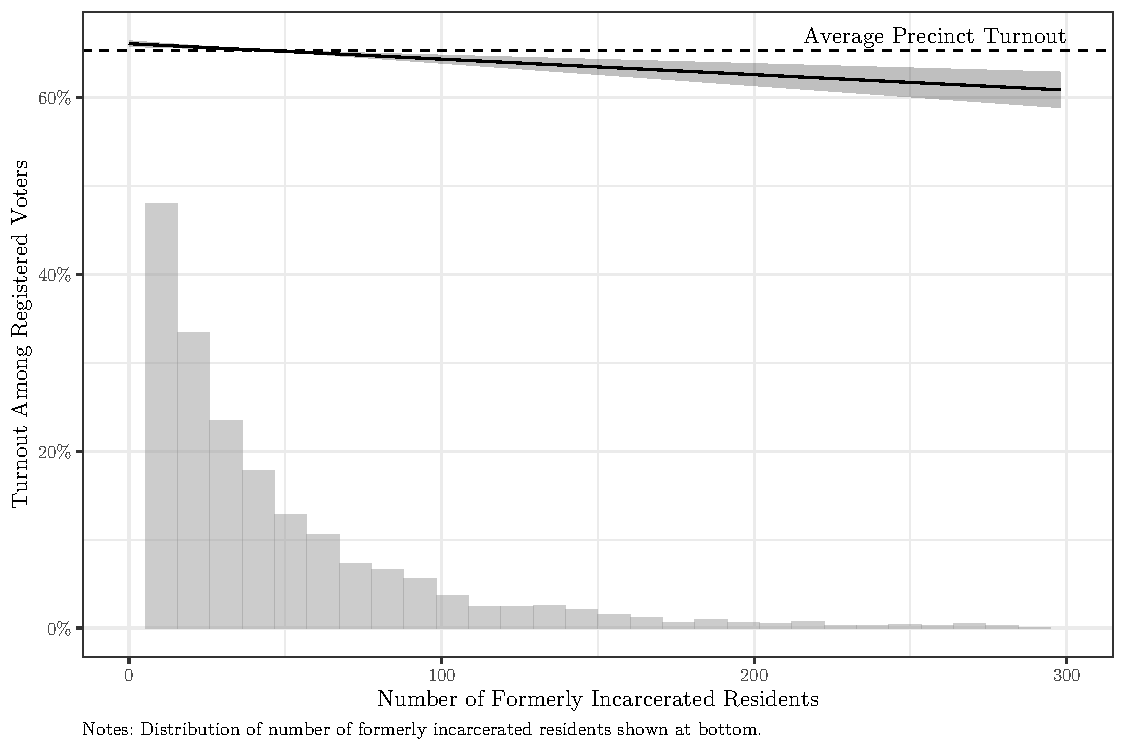
\includegraphics{amendment_4_turnout_files/figure-latex/marg1-1} 

}

\caption{\label{fig:marg1}Marginal Effect of Each Formerly Incarcerated Residents on Precinct Turnout Among Registered Voters}\label{fig:marg1}
\end{figure}

The precinct-level data allows me to test for other relationships between the number of formerly incarcerated residents in a neighborhood, the length of time since residents were released from prison, and that neighborhood's engagement with Amendment 4. In Table \ref{tab:other-precincts} I present the results of OLS models that test whether the number of formerly incarcerated community members influences a neighborhood's support for Amendment 4 or Amendment 4 roll-off. Roll-off is calculated as \(1 - \frac{Ballots\:Cast\:for\:Amendment\:4}{Ballots\:Cast\:in\:Contest\:with\:the\:Most\:Votes}\). It ranges from zero (if everyone who cast a ballot made a decision on the Amendment 4 question) to one (if no participants voted for or against Amendment 4). A lower number, therefore, represents lower roll-off and higher engagement.

\begin{singlespace}

\input{"../temp/precinct_other.tex"}
\end{singlespace}

Table \ref{tab:other-precincts} demonstrates that, although Amendment 4 did not boost precinct-level turnout, precincts with more formerly incarcerated residents \emph{did} support Amendment 4 at slightly higher rates. Similarly, roll-off was lower in neighborhoods with more formerly incarcerated resident. Thus it appears that while the presence of formerly incarcerated individuals in a neighborhood was not associated with getting people into the voting booth, it was associated with how voters cast their ballots once there. These models support hypotheses 2 and 3.

Figures \ref{fig:marg-alt} and \ref{fig:marg-alt2} plot the marginal effect of each additional formerly incarcerated resident on a precinct's support for Amendment 4 (model 1), and the precinct's roll-off on Amendment 4 (model 3). These figures make clear that the number of formerly incarcerated residents has a relatively small impact on precinct support for its passage, and a relatively large impact on precinct level roll-off.

\begin{figure}[H]

{\centering 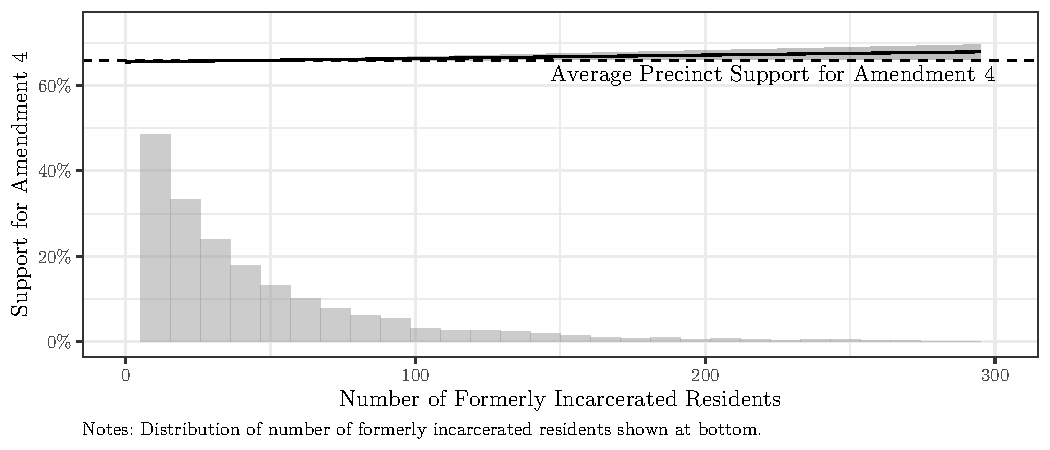
\includegraphics{amendment_4_turnout_files/figure-latex/marg-alt-1} 

}

\caption{\label{fig:marg-alt}Marginal Effect of Formerly Incarcerated Residents on Support for Amendment 4}\label{fig:marg-alt}
\end{figure}
\begin{figure}[H]

{\centering 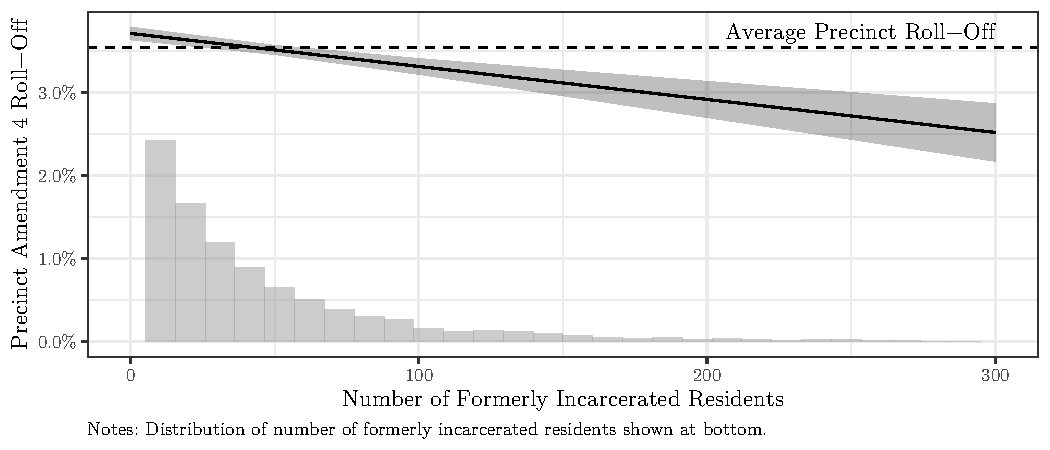
\includegraphics{amendment_4_turnout_files/figure-latex/marg-alt2-1} 

}

\caption{\label{fig:marg-alt2}Marginal Effect of Formerly Incarcerated Residents on Amendment 4 Roll-Off}\label{fig:marg-alt2}
\end{figure}

As expected, the number of formerly incarcerated individuals was highly correlated with roll-off. The issue of voting rights restoration is clearly more salient in neighborhoods where a larger share of the population would be affected. Why the relationship between formerly incarcerated residents and support is less strong (though positive) is not as clear, perhaps pointing to a variety of individual responses to crime and criminal justice policy in these neighborhoods. As Leverentz (\protect\hyperlink{ref-Leverentz2011}{2011}) argues, punitiveness is positively correlated with the salience of crime; therefore, the presence of recently incarcerated residents might activate both punitiveness and support for the amendment, with support winning out slightly.

Neighborhoods where the average formerly incarcerated resident has been out of prison for longer saw both higher support for Amendment 4 and higher roll-off. It is unsurprising that the ballot initiative is less salient in areas with less-recent incarcerations. Further, it is possible that temporal removal from the return of a resident from prison erodes punitiveness more quickly than support, leading to overall higher support for Amendment 4 where individuals have been out of prison longer. Ultimately, the data at hand cannot directly test these hypotheses; future work ought to directly interrogate these relationships.

\hypertarget{individual-level-results}{%
\subsection*{Individual-Level Results}\label{individual-level-results}}
\addcontentsline{toc}{subsection}{Individual-Level Results}

Thus far I have established that neighborhoods with more formerly incarcerated residents turned out at lower rates than other neighborhoods. By controlling for historical neighborhood turnout, the negative spillover effects of felony disenfranchisement should have been incorporated into the baseline. That turnout was lower in 2018 even after controlling for historical spillover effects is sobering, indicating imperviousness in these neighborhoods to the conditions that led to high turnout across the state.

The use of neighborhood data, however, can obscure underlying patterns. Inducements to vote at the household level might be too small to register at the neighborhood level. It is possible that Amendment 4 shaped turnout differently for individuals who cohabitate with formerly incarcerated individuals than for their neighbors. A neighborhood may have disengaged from the political process thanks to a history of aggressive state action. Household members of the formerly incarcerated may have had a similar historical response, and yet be more susceptible to mobilization from Amendment 4; they are, after all, the individuals whose identities are most likely shaped by proximity to felony disenfranchisement. The presence of formerly incarcerated individuals may have successfully mobilized household members but not neighbors.

Using individual-level data, I here distinguish the effect of proximal neighborhood contact from individual contact on turnout in 2018. As discussed above, I identify individuals who live with formerly incarcerated individuals by matching addresses listed in the Department of Corrections release data to the registered voter file. All registered voters who live at an address reported by a formerly incarcerated individual are considered ``treated.''

Each treated individual is then matched with five untreated registered voters elsewhere in her congressional district.\footnote{Due to computing constraints, a random 5 percent random sample stratified by treatment status is used to calculate the genetic weights. The full sample is used for matching.} I use five matches in order to increase the sample size of the study; the large pool of potential controls means this can be done without sacrificing the quality of the matches. Exact matching is done on all characteristics with the exception of registration date, age, median income, and share with some collegiate education, and matching is done with replacement. Ties are not broken, which means that some treated voters may have more than five controls; the regression weights are calculated to allow for this possibility. Voters are matched using their block group's median income and share with some collegiate education (from the ACS 5 year estimates ending in 2018), while all other characteristics come from the individual-level voter file.

Table \ref{tab:bal-table} presents the results of the matching exercise. In addition to the characteristics reported in Table \ref{tab:bal-table}, matches are required to come from the same congressional district to account for levels of congressional competition in the 2018 election.

\begin{singlespace}
\begin{table}[H]

\caption{\label{tab:balance-tab-chunk}\label{tab:bal-table} Balance Table}
\centering
\resizebox{\linewidth}{!}{
\begin{tabular}[t]{lllllrrrr}
\toprule
\multicolumn{1}{c}{ } & \multicolumn{2}{c}{Means: Unmatched Data} & \multicolumn{2}{c}{Means: Matched Data} & \multicolumn{4}{c}{Percent Improvement} \\
\cmidrule(l{3pt}r{3pt}){2-3} \cmidrule(l{3pt}r{3pt}){4-5} \cmidrule(l{3pt}r{3pt}){6-9}
 & Treated & Control & Treated & Control & Mean Diff & eQQ Med & eQQ Mean & eQQ Max\\
\midrule
\%White & 41.5\% & 63.2\% & 41.5\% & 41.5\% & 100.00 & 100.00 & 100.00 & 100.00\\
\% Black & 38.8\% & 12.7\% & 38.8\% & 38.8\% & 100.00 & 100.00 & 100.00 & 100.00\\
\% Latino & 12.8\% & 16.9\% & 12.8\% & 12.9\% & 99.86 & 99.86 & 99.86 & 99.86\\
\% Asian & 0.8\% & 2.0\% & 0.8\% & 0.8\% & 100.00 & 100.00 & 100.00 & 100.00\\
\% Female & 55.2\% & 52.4\% & 55.2\% & 55.2\% & 100.00 & 100.00 & 100.00 & 100.00\\
\% Male & 41.5\% & 45.0\% & 41.5\% & 41.5\% & 99.74 & 99.74 & 99.74 & 99.74\\
Registration Date & 2004-01-28 & 2004-09-24 & 2004-01-28 & 2004-02-10 & 94.63 & 30.85 & 20.67 & 16.86\\
Age & 48.95 & 52.45 & 48.95 & 48.82 & 96.12 & 95.63 & 93.77 & 91.93\\
\% Democrat & 53.7\% & 36.9\% & 53.7\% & 53.7\% & 100.00 & 100.00 & 100.00 & 100.00\\
\% Republican & 21.0\% & 35.4\% & 21.0\% & 21.0\% & 100.00 & 100.00 & 100.00 & 100.00\\
\% with Some College & 66.5\% & 75.3\% & 66.5\% & 66.5\% & 99.88 & 99.93 & 99.89 & 99.54\\
Median Income & \$47,389 & \$62,995 & \$47,389 & \$47,401 & 99.93 & 99.85 & 99.76 & 99.32\\
\bottomrule
\end{tabular}}
\end{table}
\end{singlespace}

As Table \ref{tab:bal-table} makes clear, the treated registered voters differ in meaningful ways from the rest of the electorate: they are three times as likely to be Black, they are substantially more likely to be registered as Democrats, and they live in neighborhoods with lower incomes. The matching process, however, results in a control group that is very similar to the treatment group; in each measure, there was at least a 94 percent improvement in the mean difference.

After matching the treated voters to appropriate controls, I construct a difference-in-differences model. Before presenting the results of the model, I show in Figure \ref{fig:dind} that the parallel trends assumption is satisfied: although the treatment group has lower turnout rates in general, the gap between the treatment and control groups is largely constant between 2010 and 2016.

Turnout in each year is measured among voters registered in 2018. Later years show higher turnout in part because some voters who cast ballots in the earlier elections were no longer registered in 2018. Voters who registered late in the period, on the other hand, are included in the denominator each year. By including registration date in the matching procedure I control directly for potential differences in registration timing between treated and control voters. Of course, some of the increase in turnout observed in later years in Figure \ref{fig:dind} can be attributed to higher ``real'' turnout as a share of eligible citizens.

\begin{figure}[H]

{\centering 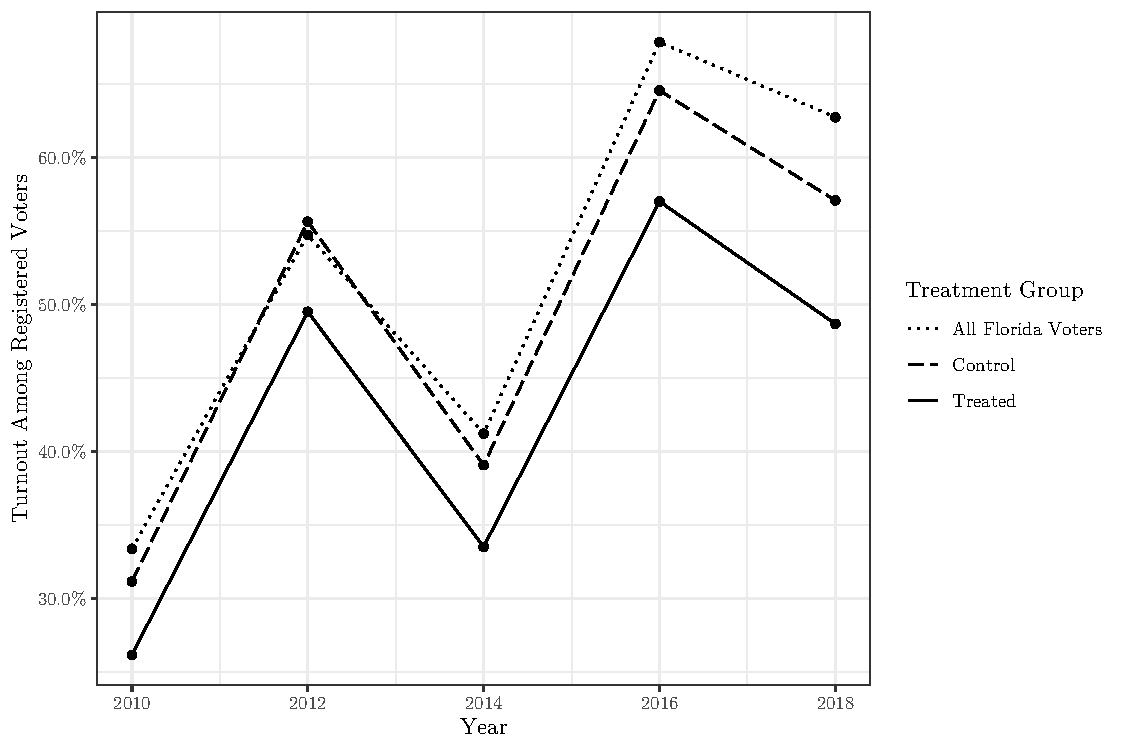
\includegraphics{amendment_4_turnout_files/figure-latex/dind-1} 

}

\caption{\label{fig:dind}General Election Turnout for Treated and Control Voters, 2010 -- 2018}\label{fig:dind}
\end{figure}

The trends presented in Figure \ref{fig:dind} offer preliminary visual corroboration of what I find at the neighborhood level --- namely, that 2018 turnout was not higher for voters in proximal contact with formerly incarcerated individuals. Table \ref{tab:tab-dind} formalizes these trends into an ordinary least squares regression.\footnote{Although the dependent variable here is binary --- it takes the value 0 if a voter does not participate, and 1 if she does --- the coefficients produced by logistic regressions in the difference-in-differences context are largely uninterpretable. I thus use a linear specification here. When the models are estimated using a logistic specification, the treatment effect is virtually identical.} A treatment dummy distinguishes treated from control voters. The treatment dummy is interacted with another dummy identifying the 2018 election. Robust standard errors are clustered at the level of the match (Abadie and Spiess \protect\hyperlink{ref-Abadie2019}{2019}). Model 1 presents the model output without the other controls used for matching; Model 2 includes these covariates.

In models 3 and 4 of Table \ref{tab:tab-dind} I consider the possibility that, as households become further removed from a member's incarceration, the negative effects of their incarceration on turnout dissipate. In these models, the dummies indicating treatment and the 2018 election are interacted with the number of years since the most recent completion of a term of incarceration for a household member (\emph{Years Since Latest Incarceration}, shortened to \emph{Years Since} in interactions). Matched control observations are assigned the value associated with their treated observation. Model 3 includes no other covariates, while Model 4 includes the matched variables.

It is, of course, highly possible that formerly incarcerated individuals no longer live in the same household they reported when leaving prison. This is especially true for individuals released from prison early in the sample. To control for this possibility, Models 5 -- 8 include only the treated individuals (and their matches) whose registration dates are earlier than the latest prison release date of a household member. These are individuals, therefore, that we can be relatively sure lived with an incarcerated individual. The treatment effects in these models, though slightly larger, tell the same general story.

\begin{singlespace}
\input{"../temp/dind_reg.tex"}
\end{singlespace}

Each of the specifications presented in Table \ref{tab:tab-dind} identify a negative treatment effect. The coefficients on \emph{2018 × Treated} in Models 1 and 2 indicate that turnout among treated voters was about 2.3 percentage points below what it would have been if the gap between treated and control voters in 2018 had conformed to prior years.

There is some indication that ``spillover'' effects lessen over time. In each model, \emph{2018 × Treated × Years Since} and \emph{Treated × Years Since} is positive and statistically significant. In other words, individuals who lived with housemates who had not been imprisoned in many years were more likely to vote than other treated voters, and this was especially true in 2018. Models 3 and 4 estimate that the treatment effect for individuals whose household member returned from prison within one year of the election was about -3.9 percentage points, but that for each year the most recent incarceration recedes into the past, the treatment effect decreases by about 0.2 points in years other than 2018, and by 0.4 points in 2018. That the spillover effects ``decay'' is a positive sign, and indicates that the negative socialization induced by a housemate's incarceration might not be permanent. It is also possible that incarcerations occurring in different historical periods like the late 1990s were interpreted differently and had smaller spillover effects.

That the effect is moderated by time is unsurprising. Individuals whose household members went to and were released from prison between the 2016 and 2018 elections, for instance, received two treatments: they both were ``negatively'' treated by their proximal contact with the criminal justice system and potentially ``positively'' treated by Amendment 4. What \emph{is} surprising, however, is the continued negative treatment effect even for the households that were most removed from their proximal contact with the incarceration of a household member. Table \ref{tab:oldies} presents the results of Models 5 and 6 from Table \ref{tab:tab-dind}, but limits the pool to households where the most recent incarceration ended prior to 2010. The negative shock of proximal contact for these individuals should be reflected in the base years of the difference-in-differences models. That \emph{2018 × Treated} remains significant and negative for these individuals is puzzling.

\begin{singlespace}
\input{"../temp/dind_reg_medium.tex"}
\end{singlespace}

This negative, significant finding for treated individuals whose household members had been out of prison for many years should probably not be interpreted to mean that Amendment 4 had a demobilizing effect on individuals in proximal contact to formerly incarcerated individuals. Rather, it likely points to meaningful differences in susceptibility to broad mobilization for those in proximal contact with the criminal justice system. As discussed above, the 2018 election was historic in many ways with higher turnout than any midterm in a century. Many marginal voters who had not previously participated in midterm elections turned out.

And yet, this negative treatment effect is troubling. As Table \ref{tab:bal-table} indicates, the matching procedure was successful at creating a control group that looks nearly identical to the treatment group according to observable characteristics, though Figure \ref{fig:dind} shows that treated voters historically turn out at low rates. Not only did Amendment 4 fail to mobilize voters who live in close proximity to the formerly incarcerated; it appears that these voters are also \emph{less} mobilized by the same factors that encourage similar voters to participate in unique elections such as that of 2018. This analysis cannot determine whether the proximal contact caused this imperviousness to broadly mobilizing conditions, or if individuals who live in close proximity to the formerly incarcerated would have been more likely to remain on the sidelines in an election like 2018 even without the proximal contact in their past. Nevertheless, their relatively depressed turnout in 2018 --- even with Amendment 4 on the ballot --- underscores just how difficult their political (re)integration is.

\hypertarget{discussion-and-conclusion}{%
\subsection*{Discussion and Conclusion}\label{discussion-and-conclusion}}
\addcontentsline{toc}{subsection}{Discussion and Conclusion}

Turnout in 2018 hit historic levels for a midterm election as infrequent voters participated and made their voices heard. In addition to hotly contested Congressional, senate, and gubernatorial races, Floridians were presented with the opportunity to restore voting rights to well over a million permanently disenfranchised individuals who had been convicted of felony offenses. Amendment 4 and its organizers were hugely successful --- in a year where both statewide winners won by less than 0.5 percentage points, nearly two-thirds of Floridians supported expanding the franchise. Neighborhoods and voters most directly impacted by felony disenfranchisement stood to gain meaningful political representation from the passage of the amendment, and one of the ``durable markers'' of their civil death was nullified. And these proximal voters \emph{did} turn out at higher rates in 2018 than in previous elections: turnout among treated voters registered as of the 2014 midterm increased from 41.5 percent that year to 52.5 percent in 2018. And the presence of formerly incarcerated individuals measurably increased the degree to which a neighborhood supported and engaged with the amendment.

Despite these major gains in turnout among individuals in proximate contact with the carceral state, I fail to uncover evidence that Amendment 4 itself increased the turnout among these individuals above-and-beyond the increases observed among other voters and in other communities. Although the substance of the amendment and language used to promote it spoke of a reconciled citizenship, they were not more likely to participate. In fact, the evidence points in the opposite direction: turnout for these voters actually increased \emph{less} in 2018 than it did for other voters. Not only was Amendment 4 not particularly mobilizing, but these voters are also less susceptible to factors contributing to statewide surges in turnout. However, the strong relationship between roll-off and the number of formerly incarcerated residents implies that the rights restoration was highly salient for the voters who did cast a ballot.

Why Amendment 4 did not mobilize these voters is not immediately apparent. It could be an issue of voter knowledge: previous research has indicated that marginalized voters demonstrate lower political knowledge (Erikson \protect\hyperlink{ref-Erikson2015}{2015}). If these proximal contact voters were not aware that Amendment 4 was on the ballot, the amendment could hardly have mobilized them to vote. Although the campaign in support of the amendment was very large, the Florida Rights Restoration Coalition may have focused on contacting higher propensity voters, even though these voters were less likely to directly benefit from the passage of the amendment. Further research is needed to understand how and why these communities were not more likely to vote than their counterparts.

Whatever the causal mechanism that resulted in lower turnout for these communities despite Amendment 4, the results point to the next chapter of the fight for political integration and representation for advocates in the Sunshine State. The relatively lower turnout in 2018 for the communities most impacted by the carceral state indicates that formal re-enfranchisement is not enough. If Floridian and American democracy wants to \emph{actually} incorporate voices from these communities --- and not simply legally \emph{allow} for their incorporation --- the advocacy movement cannot consider its work done once the formal barriers to the ballot box have been torn down. Re-enfranchisement is clearly necessary, but it is not sufficient. Researchers must continue exploring why the political re-incorporation of these communities is so difficult, and advocates on the ground must do the hard work of reknitting them to our body politic.

The questions raised by this manuscript are especially important considering the fight over Amendment 4 that has played out in federal court. Just months after the 2018 election the Florida legislature passed a bill requiring disenfranchised individuals to pay off all court-ordered financial obligations before registering to vote, despite the fact that the state seemed incapable of actually determining how much any individual actually owed (Stern \protect\hyperlink{ref-Stern2019}{2019}). In May of 2020, a federal judge ruled the law unconstitutional, arguing that conditioning voting rights on the repayment of obligations that individuals cannot afford amounts to a poll tax and violation of the 24th Amendment.\footnote{Jones et al.~v. DeSantis et al., 4:19cv300-RH/MJF (U.S. District Court for the Northern District of Florida 2020).} In September 2020, however, the U.S. Court of Appeals for the 11th Circuit overturned that decision,\footnote{Jones et al.~v. DeSantis et al., 4:19cv300-RH/MJF (United States Court of Appeals for the Eleventh Circuit).} upholding the constitutionality of the law. In his dissent, Judge Adalberto Jordan argued that ``{[}h{]}ad Florida wanted to create a system to obstruct, impede, and impair the ability of felons to vote under Amendment 4, it could not have come up with a better one'' and that ``Florida cannot tell felons --- the great majority of whom are indigent --- how much they owe\ldots{} and has come up with conflicting (and uncodified) methods for determining how LFO payments by felons should be credited.'' That Florida legislators would condition voting on criteria that cannot be verified, or cannot be afforded, has understandably been described as ``unfair {[}and{]} heartbreaking'' by one disenfranchised individual who said the amendment had promised to ``give me a voice in my own future'' (Harris \protect\hyperlink{ref-Harris2020}{2020}). It remains to be seen how such legislation and litigation will inform how criminal justice-involved individuals understand their relationship with the state and structure their future democratic participation.

\newpage

\hypertarget{references}{%
\subsection*{References}\label{references}}
\addcontentsline{toc}{subsection}{References}

\hypertarget{refs}{}
\begin{cslreferences}
\leavevmode\hypertarget{ref-Abadie2019}{}%
Abadie, Alberto, and Jann Spiess. 2019. ``Robust Post-Matching Inference.'' \emph{Working Paper.}

\leavevmode\hypertarget{ref-Amos2020}{}%
Amos, Brian, and Michael P. McDonald. 2020. ``A Method to Audit the Assignment of Registered Voters to Districts and Precincts.'' \emph{Political Analysis}, 1--16. \url{https://doi.org/10.1017/pan.2019.44}.

\leavevmode\hypertarget{ref-Amos2017}{}%
Amos, Brian, Michael P. McDonald, and Russell Watkins. 2017. ``When Boundaries CollideConstructing a National Database of Demographic and Voting Statistics.'' \emph{Public Opinion Quarterly} 81 (S1): 385--400. \url{https://doi.org/10.1093/poq/nfx001}.

\leavevmode\hypertarget{ref-Austin2004}{}%
Austin, Regina. 2004. ``The Shame of It All: Stigma and the Political Disenfranchisement of Formerly Convicted and Incarcerated Persons Symposium on Race, Crime, and Voting: Social, Political, and Philosophical Perspectives on Felony Disenfranchisement in America.'' \emph{Columbia Human Rights Law Review} 36 (1): 173--92. \url{https://heinonline.org/HOL/P?h=hein.journals/colhr36\&i=181}.

\leavevmode\hypertarget{ref-Baumann2019}{}%
Baumann, Joella. 2019. ``Paroled Coloradans Are Now Eligible to Vote.'' \emph{Colorado Public Radio}, July 1, 2019. \url{https://www.cpr.org/2019/07/01/paroled-coloradans-are-now-eligible-to-vote/}.

\leavevmode\hypertarget{ref-Berman2018}{}%
Berman, Ari. 2018. ``Inside the Unlikely Movement That Could Restore Voting Rights to 1.4 Million Floridians.'' \emph{Mother Jones: Politics}, November 2018. \url{https://www.motherjones.com/politics/2018/10/inside-the-unlikely-movement-that-could-restore-voting-rights-to-1-4-million-floridians/}.

\leavevmode\hypertarget{ref-Bousquet2018a}{}%
Bousquet, Steve. 2018. ``Judge: Florida's Early Voting-on-Campus Ban Shows `Stark Pattern of Discrimination'.'' \emph{Tampa Bay Times}, July 24, 2018. \url{https://www.tampabay.comundefined/}.

\leavevmode\hypertarget{ref-Bowers2009}{}%
Bowers, Melanie, and Robert R. Preuhs. 2009. ``Collateral Consequences of a Collateral Penalty: The Negative Effect of Felon Disenfranchisement Laws on the Political Participation of Nonfelons*.'' \emph{Social Science Quarterly} 90 (3): 722--43. \url{https://doi.org/10.1111/j.1540-6237.2009.00640.x}.

\leavevmode\hypertarget{ref-Bullock1996}{}%
Bullock, Charles S., and Richard E. Dunn. 1996. ``Election Roll-Off: A Test of Three Explanations.'' \emph{Urban Affairs Review} 32 (1): 71--86. \url{https://doi.org/10.1177/107808749603200104}.

\leavevmode\hypertarget{ref-Burch2011}{}%
Burch, Traci. 2011. ``Turnout and Party Registration Among Criminal Offenders in the 2008 General Election.'' \emph{Law \& Society Review} 45 (3): 699--730. \url{https://doi.org/10.1111/j.1540-5893.2011.00448.x}.

\leavevmode\hypertarget{ref-Burch2013}{}%
Burch, Traci R. 2013. ``Effects of Imprisonment and Community Supervision on Neighborhood Political Participation in North Carolina:'' \emph{The ANNALS of the American Academy of Political and Social Science}, November. \url{https://doi.org/10.1177/0002716213503093}.

\leavevmode\hypertarget{ref-Bushway2007}{}%
Bushway, Shawn D., Michael A. Stoll, and David Weiman. 2007. \emph{Barriers to Reentry?: The Labor Market for Released Prisoners in Post-Industrial America}. Russell Sage Foundation. \url{http://books.google.com?id=YOeFAwAAQBAJ}.

\leavevmode\hypertarget{ref-Erikson2015}{}%
Erikson, Robert S. 2015. ``Income Inequality and Policy Responsiveness.'' \emph{Annual Review of Political Science} 18 (1): 11--29. \url{https://doi.org/10.1146/annurev-polisci-020614-094706}.

\leavevmode\hypertarget{ref-Ewald2002}{}%
Ewald, A.c. 2002. ``"Civil Death": The Ideological Paradox of Criminal Disenfranchisement Law in the United States.'' \emph{Wisconsin Law Review} 2002 (5): 1045--1137. \url{http://proxy.library.nyu.edu/login?url=http://search.ebscohost.com/login.aspx?direct=true\&db=edselc\&AN=edselc.2-52.0-0036997235\&site=eds-live}.

\leavevmode\hypertarget{ref-Gelman2007}{}%
Gelman, Andrew, Jeffrey Fagan, and Alex Kiss. 2007. ``An Analysis of the New York City Police Department's `Stop-and-Frisk' Policy in the Context of Claims of Racial Bias.'' \emph{Journal of the American Statistical Association} 102 (479): 813--23. \url{https://doi.org/10.1198/016214506000001040}.

\leavevmode\hypertarget{ref-Harris2020}{}%
Harris, Alex. 2020. ``Losing Vote After Amendment 4 Win Is Unfair, Heartbreaking.'' \emph{Orlando Sentinel}, August 7, 2020. \url{https://www.orlandosentinel.com/opinion/guest-commentary/os-op-limiting-amendment-4-is-a-setback-20200807-hvcef76xongytccvyivu7o4s3y-story.html}.

\leavevmode\hypertarget{ref-Kelso2018}{}%
Kelso, Nathaniel, and Michael Migurski. 2018. ``Election-Geodata.'' 2018. \url{https://github.com/nvkelso/election-geodata}.

\leavevmode\hypertarget{ref-Kilgore2018}{}%
Kilgore, Ed. 2018. ``2018 Turnout Was the Highest of Any Midterm in More Than a Century.'' Intelligencer. November 13, 2018. \url{https://nymag.com/intelligencer/2018/11/2018-turnout-was-the-highest-of-any-midterm-since-1914.html}.

\leavevmode\hypertarget{ref-King2016}{}%
King, Bridgett A., and Laura Erickson. 2016. ``Disenfranchising the Enfranchised: Exploring the Relationship Between Felony Disenfranchisement and African American Voter Turnout.'' \emph{Journal of Black Studies}, July. \url{https://doi.org/10.1177/0021934716659195}.

\leavevmode\hypertarget{ref-Knack2008}{}%
Knack, Stephen, and Martha Kropf. 2008. ``Roll-Off at the Top of the Ballot: International Undervoting in American Presidential Elections.'' \emph{Politics \& Policy} 31 (4): 575--94. \url{https://doi.org/10.1111/j.1747-1346.2003.tb00163.x}.

\leavevmode\hypertarget{ref-Lerman2013}{}%
Lerman, Amy E., and Vesla Weaver. 2013. ``Staying Out of Sight? Concentrated Policing and Local Political Action:'' \emph{The ANNALS of the American Academy of Political and Social Science}, November. \url{https://doi.org/10.1177/0002716213503085}.

\leavevmode\hypertarget{ref-Lerman2014}{}%
Lerman, Amy E., and Vesla M. Weaver. 2014. \emph{Arresting Citizenship: The Democratic Consequences of American Crime Control}. Chicago Studies in American Politics. Chicago ; London: The University of Chicago Press.

\leavevmode\hypertarget{ref-Leverentz2011}{}%
Leverentz, Andrea. 2011. ``Neighborhood Context of Attitudes Toward Crime and Reentry.'' \emph{Punishment \& Society} 13 (1): 64--92. \url{https://doi.org/10.1177/1462474510385629}.

\leavevmode\hypertarget{ref-Martin2018}{}%
Martin, Karin D., Bryan L. Sykes, Sarah Shannon, Frank Edwards, and Alexes Harris. 2018. ``Monetary Sanctions: Legal Financial Obligations in US Systems of Justice.'' \emph{Annual Review of Criminology} 1 (1): 471--95. \url{https://doi.org/10.1146/annurev-criminol-032317-091915}.

\leavevmode\hypertarget{ref-McDonald2002}{}%
McDonald, Michael P. 2002. ``The Turnout Rate Among Eligible Voters in the States, 1980--2000.'' \emph{State Politics \& Policy Quarterly} 2 (2): 199--212. \url{https://doi.org/10.1177/153244000200200205}.

\leavevmode\hypertarget{ref-Merolla2013}{}%
Merolla, Jennifer L., Abbylin H. Sellers, and Derek J. Fowler. 2013. ``Descriptive Representation, Political Efficacy, and African Americans in the 2008 Presidential Election.'' \emph{Political Psychology} 34 (6): 863--75. \url{https://doi.org/10.1111/j.1467-9221.2012.00934.x}.

\leavevmode\hypertarget{ref-Mettler2002}{}%
Mettler, Suzanne. 2002. ``Bringing the State Back in to Civic Engagement: Policy Feedback Effects of the G.I. Bill for World War II Veterans.'' \emph{The American Political Science Review} 96 (2): 351--65. \url{http://www.jstor.org/stable/3118030}.

\leavevmode\hypertarget{ref-Mettler2004}{}%
Mettler, Suzanne, and Joe Soss. 2004. ``The Consequences of Public Policy for Democratic Citizenship: Bridging Policy Studies and Mass Politics.'' \emph{Perspectives on Politics} 2 (1): 55--73. \url{http://www.jstor.org/stable/3688340}.

\leavevmode\hypertarget{ref-Miles2004}{}%
Miles, Thomas J. 2004. ``Felon Disenfranchisement and Voter Turnout.'' \emph{The Journal of Legal Studies} 33 (1): 85--129. \url{https://doi.org/10.1086/381290}.

\leavevmode\hypertarget{ref-Miller2016}{}%
Miller, Bryan Lee, and Laura E. Agnich. 2016. ``Unpaid Debt to Society: Exploring How Ex-Felons View Restrictions on Voting Rights After the Completion of Their Sentence.'' \emph{Contemporary Justice Review} 19 (1): 69--85. \url{https://doi.org/10.1080/10282580.2015.1101685}.

\leavevmode\hypertarget{ref-Miller2012}{}%
Miller, Bryan Lee, and Joseph F. Spillane. 2012a. ``Civil Death: An Examination of Ex-Felon Disenfranchisement and Reintegration:'' \emph{Punishment \& Society}, October. \url{https://doi.org/10.1177/1462474512452513}.

\leavevmode\hypertarget{ref-Miller2012a}{}%
---------. 2012b. ``Governing the Restoration of Civil Rights for Ex-Felons: An Evaluation of the Executive Clemency Board in Florida.'' \emph{Contemporary Justice Review} 15 (4): 413--34. \url{https://doi.org/10.1080/10282580.2012.734568}.

\leavevmode\hypertarget{ref-Morris2020}{}%
Morris, Kevin. 2020. ``Neighborhoods and Felony Disenfranchisement: The Case of New York City.'' \emph{Urban Affairs Review}, May, 1078087420921522. \url{https://doi.org/10.1177/1078087420921522}.

\leavevmode\hypertarget{ref-Naser2006}{}%
Naser, Rebecca L, and Christy A Visher. 2006. ``Family Members' Experiences with Incarceration and Reentry.'' \emph{Western Criminology Review} 7 (2): 20--31.

\leavevmode\hypertarget{ref-ORLANDOSENTINEL2018}{}%
\emph{Orlando Sentinel}. 2018. ``Florida's Election 2018: Our Endorsements for Governor, U.S. Senate, U.S. House and the Amendments,'' October 19, 2018. \url{https://www.orlandosentinel.com/opinion/editorials/os-op-orlando-sentinel-endorsements-20181018-htmlstory.html\#amend4\%5D}.

\leavevmode\hypertarget{ref-Ramadan2018}{}%
Ramadan, Lulu, Mike Stucka, and Wayne Washington. 2018. ``Florida Felon Voting Rights: Who Got Theirs Back Under Scott?'' \emph{The Palm Beach Post}, October 25, 2018. \url{https://www.palmbeachpost.com/news/20181025/florida-felon-voting-rights-who-got-theirs-back-under-scott}.

\leavevmode\hypertarget{ref-Robles2018}{}%
Robles, Frances. 2018. ``1.4 Million Floridians with Felonies Win Long-Denied Right to Vote.'' \emph{The New York Times: U.S.}, November 7, 2018. \url{https://www.nytimes.com/2018/11/07/us/florida-felon-voting-rights.html}.

\leavevmode\hypertarget{ref-Rosenbaum2005}{}%
Rosenbaum, Dennis P., Amie M. Schuck, Sandra K. Costello, Darnell F. Hawkins, and Marianne K. Ring. 2005. ``Attitudes Toward the Police: The Effects of Direct and Vicarious Experience.'' \emph{Police Quarterly} 8 (3): 343--65. \url{https://doi.org/10.1177/1098611104271085}.

\leavevmode\hypertarget{ref-Schlakman2018}{}%
Schlakman, Mar. 2018. ``Some Facts and Figures You Might Not Know About Civil Rights Restoration in Florida.'' \emph{Tampa Bay Times}, April 19, 2018. \url{https://www.tampabay.com/opinion/columns/Column-Some-facts-and-figures-you-might-not-know-about-civil-rights-restoration-in-Florida_167477194/}.

\leavevmode\hypertarget{ref-Sekhon2011}{}%
Sekhon, Jasjeet S. 2011. ``Multivariate and Propensity Score Matching Software with Automated Balance Optimization: The Matching Package for R.'' \emph{Journal of Statistical Software} 42 (1): 1--52. \url{https://doi.org/10.18637/jss.v042.i07}.

\leavevmode\hypertarget{ref-Smith2018}{}%
Smith, Jamil. 2018. ``Andrew Gillum Is Ready. Is Florida?'' Rolling Stone. October 31, 2018. \url{https://www.rollingstone.com/politics/politics-features/andrew-gillum-florida-governor-race-749651/}.

\leavevmode\hypertarget{ref-Soss1999}{}%
Soss, Joe. 1999. ``Lessons of Welfare: Policy Design, Political Learning, and Political Action.'' \emph{The American Political Science Review} 93 (2): 363--80. \url{https://doi.org/10.2307/2585401}.

\leavevmode\hypertarget{ref-Stern2019}{}%
Stern, Mark Joseph. 2019. ``Florida Republicans Are Sabotaging a Constitutional Amendment That Gave Felons the Right to Vote.'' Slate Magazine. March 20, 2019. \url{https://slate.com/news-and-politics/2019/03/florida-republicans-felon-voting-rights-amendment-4.html}.

\leavevmode\hypertarget{ref-SunSentinelEditorial2018}{}%
\emph{Sun Sentinel}. 2018. ``Five Good --- Seven Bad --- Amendments for Florida's Constitution,'' October 5, 2018. \url{https://www.sun-sentinel.com/opinion/endorsements/fl-op-end-good-bad-constitutional-amendments-20181005-story.html}.

\leavevmode\hypertarget{ref-tampabaytimes2018}{}%
\emph{Tampa Bay Times}. 2018. ``Times Recommends: Yes on Amendment 4,'' October 3, 2018. \url{https://www.tampabay.com/opinion/editorials/times-recommends-yes-on-amendment-4-20180928/}.

\leavevmode\hypertarget{ref-Taylor2018}{}%
Taylor, Adam. 2018. ``Florida's Move to Allow Ex-Felons to Vote Brings U.S. Closer to International Election Norms.'' \emph{Washington Post: WorldViews}, November 7, 2018. \url{https://www.washingtonpost.com/world/2018/11/07/floridas-move-allow-ex-felons-vote-brings-us-closer-international-election-norms/}.

\leavevmode\hypertarget{ref-Tragos2008}{}%
Tragos, George E., and Peter A. Sartes. 2008. ``Withhold of Adjudication: What Everyone Needs to Know.'' The Florida Bar. February 1, 2008. \url{https://www.floridabar.org/the-florida-bar-journal/withhold-of-adjudication-what-everyone-needs-to-know/}.

\leavevmode\hypertarget{ref-sentencing_2016}{}%
Uggen, Christopher, Ryan Larson, and Sarah Shannon. 2016. ``6 Million Lost Voters: State-Level Estimates of Felony Disenfranchisement, 2016.'' Research report. The Sentencing Project. \url{https://www.sentencingproject.org/publications/6-million-lost-voters-state-level-estimates-felony-disenfranchisement-2016/}.

\leavevmode\hypertarget{ref-Uggen2004a}{}%
Uggen, Christopher, Jeff Manza, and Angela Behrens. 2004. ``\,`Less Than the Average Citizens': Stigma, Role Transition, and the Civic Reintegration of Convicted Felons.'' In \emph{After Crime and Punishment: Pathways to Offender Reintegration}, edited by Shad Maruna and Russell Immarigeon. Portland, OR: Willan Publishing.

\leavevmode\hypertarget{ref-USPS2015}{}%
USPS. 2015. ``Appendix C.'' Postal Addressing Standards. May 2015. \url{https://pe.usps.com/text/pub28/28apc_002.htm}.

\leavevmode\hypertarget{ref-Vanderleeuw1987}{}%
Vanderleeuw, James M., and Richard L. Engstrom. 1987. ``Race, Referendums, and Roll-Off.'' \emph{The Journal of Politics} 49 (4): 1081--92. \url{https://doi.org/10.2307/2130785}.

\leavevmode\hypertarget{ref-Walker2014}{}%
Walker, Hannah L. 2014. ``Extending the Effects of the Carceral State: Proximal Contact, Political Participation, and Race.'' \emph{Political Research Quarterly}, July. \url{https://doi.org/10.1177/1065912914542522}.

\leavevmode\hypertarget{ref-Walker2020}{}%
---------. 2020. ``Targeted: The Mobilizing Effect of Perceptions of Unfair Policing Practices.'' \emph{The Journal of Politics} 82 (1): 119--34. \url{https://doi.org/10.1086/705684}.

\leavevmode\hypertarget{ref-Walker2017}{}%
Walker, Hannah L., and Marcela García-Castañon. 2017. ``For Love and Justice: The Mobilizing of Race, Gender, and Criminal Justice Contact.'' \emph{Politics \& Gender} 13 (4): 541--68. \url{https://doi.org/10.1017/S1743923X17000198}.

\leavevmode\hypertarget{ref-Washington2006}{}%
Washington, Ebonya. 2006. ``How Black Candidates Affect Voter Turnout.'' \emph{The Quarterly Journal of Economics} 121 (3): 973--98. \url{http://www.jstor.org/stable/25098814}.

\leavevmode\hypertarget{ref-Weaver2010}{}%
Weaver, Vesla M., and Amy E. Lerman. 2010. ``Political Consequences of the Carceral State.'' \emph{American Political Science Review} 104 (4): 817--33. \url{https://doi.org/10.1017/S0003055410000456}.

\leavevmode\hypertarget{ref-White2019a}{}%
White, Ariel. 2019a. ``Family Matters? Voting Behavior in Households with Criminal Justice Contact.'' \emph{American Political Science Review} 113 (2): 607--13. \url{https://doi.org/10.1017/S0003055418000862}.

\leavevmode\hypertarget{ref-White2019}{}%
---------. 2019b. ``Misdemeanor Disenfranchisement? The Demobilizing Effects of Brief Jail Spells on Potential Voters.'' \emph{American Political Science Review} 113 (2): 311--24. \url{https://doi.org/10.1017/S000305541800093X}.

\leavevmode\hypertarget{ref-Wines2019}{}%
Wines, Michael. 2019. ``Kentucky Gives Voting Rights to Some 140,000 Former Felons.'' \emph{The New York Times: U.S.}, December 12, 2019. \url{https://www.nytimes.com/2019/12/12/us/kentucky-felons-voting-rights.html}.
\end{cslreferences}

\newpage
\pagenumbering{gobble}
\pagenumbering{arabic}

\hypertarget{appendix-a}{%
\subsection*{Appendix A}\label{appendix-a}}
\addcontentsline{toc}{subsection}{Appendix A}

As discussed in the body of this manuscript, statewide data on the residential addresses of individuals sentenced to felony probation are not available. These data are, however, available in Hillsborough County, the county in Florida with the third-highest number of formerly incarcerated individuals.\footnote{See \url{https://www.hillsclerk.com/Records-and-Reports/Public-Data-Files}.} These records go back to 1988, though I have restricted them to individuals sentenced since October 1, 1997, so that they mirror the incarceration records. I follow the same geocoding and address cleaning procedures as for the incarceration records discussed above. These data do not include unique identifiers. To avoid double-counting, only the most recent record for each unique first name, middle name, last name, and date of birth is retained. This potentially excludes different people whose names and dates of birth are identical. Individuals whose adjudication was withheld are excluded, as are individuals whose names, dates of birth, and addresses match individuals who were formerly incarcerated. This avoids double counting individuals both incarcerated and sentenced to probation.

Figure \ref{fig:scatter} plots the relationship between the number of formerly incarcerated residents and residents who have been sentenced to felony probation in each block group in Hillsborough County (scaled by population). As the figure makes clear, individuals who have been sentenced to felony probation are concentrated in the same neighborhoods where individuals live after a period of incarceration (the \emph{R\textsuperscript{2}} of the bivariate regression is 0.91). As with the marginal effects plots in the body of this manuscript, the figure does not show outlier neighborhoods but the line of best fit and \emph{R\textsuperscript{2}} are calculated using all observations.

\begin{figure}[H]

{\centering 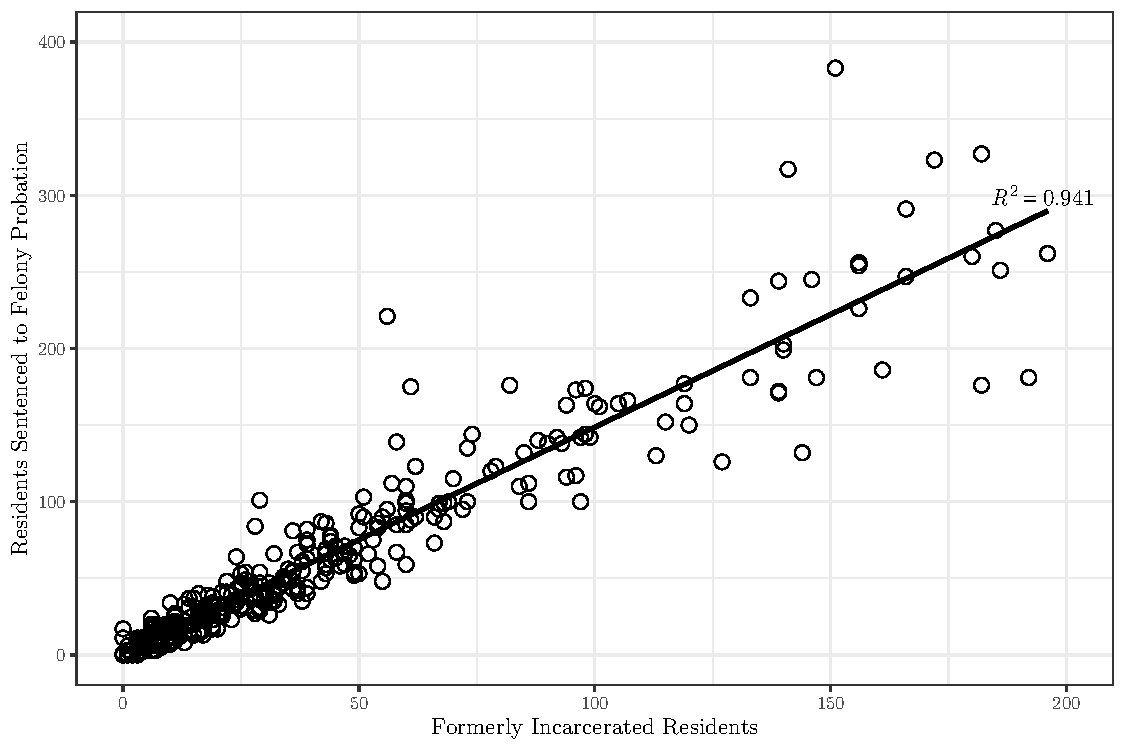
\includegraphics{amendment_4_turnout_files/figure-latex/corrplot-1} 

}

\caption{\label{fig:scatter}Relationship Between Formerly Incarcerated and Probationed Residents, Hillsborough County}\label{fig:corrplot}
\end{figure}

Table \ref{tab:ap-hills-1} replicates the models from Tables \ref{tab:to-precinct} and \ref{tab:other-precincts} in the main body of this manuscript. In each pair of models in the table, I begin by re-fitting the exact models presented in the body of this manuscript but limiting the precincts and block groups to Hillsborough County. In the second model in each pair, the primary dependent variable includes both formerly incarcerated residents \emph{and} the number of residents who have been convicted of a felony probation.

\begin{singlespace}

\input{"../temp/hills_hood.tex"}
\end{singlespace}

The relationship between disenfranchised residents and precinct-level support for Amendment 4, and precinct-level turnout, are nonsignificant in Table \ref{tab:ap-hills-1} despite being significant statewide. Block group-level turnout and roll-off remain negatively associated with the presence of disenfranchised individuals. Importantly, in no model does moving from measuring only formerly incarcerated individuals to measuring all disenfranchised individuals change the sign on a statistically significant relationship. This provides corroboration for the argument that the neighborhood-level results presented in the body of this manuscript, measured using only formerly incarcerated residents, apply to the formerly disenfranchised population more generally.

I next interrogate whether the use of only incarceration records is likely impacting the individual-level analyses presented in the body of the manuscript. I begin by re-estimating Models 1 -- 4 from Table \ref{tab:tab-dind}, limiting the pool to treated voters who live in Hillsborough County and their matches. Re-estimating the model in Hillsborough County allows us to observe how often ``unidentified'' treated voters serve as controls in this manuscript's primary analysis, at least in Hillsborough County. Approximately 6.8 percent of the controls for Hillsborough County in the primary analysis are actually household members of individuals disenfranchised due to a term of felony probation. Because voters who are in fact treated serve as controls for some registered voters living with formerly incarcerated individuals, this manuscript likely understates the effect of living with a disenfranchised individual.

I then re-run the matching procedure described above, where a registered voter is considered treated if they lived with any disenfranchised individual. Potential controls for this matching procedure are limited to Hillsborough County, where we can be sure registered voters do not live with individuals sentenced to felony probation. The matching procedure is successful at reducing differences between treated and control voters in Hillsborough County.

In Table \ref{tab:ap-hills-2}, models 1 -- 4 re-estimate models 1 -- 4 from Table \ref{tab:tab-dind}. Models 5 -- 8 present the results using the broader treatment definition.

\begin{singlespace}
\input{"../temp/dind_reg_hills.tex"}
\end{singlespace}

In Hillsborough County, the magnitude of the treatment effect grows when we broaden the treatment group to include anyone who lives with a formerly disenfranchised individual. This raises interesting questions about the potential differential spillover effects of living with a formerly incarcerated individual versus with an individual sentenced to felony probation. This may also be due to some housemates of probationed individuals serving as controls in the main analysis, collapsing the distinction between treated and control and producing conservative estimates. Nonetheless, Table \ref{tab:ap-hills-2} provides evidence that the negative treatment effects identified among voters living with formerly incarcerated individuals in the body of this manuscript are likely generalizeable to all voters living with disenfranchised individuals.

\newpage

\hypertarget{appendix-b}{%
\subsection*{Appendix B}\label{appendix-b}}
\addcontentsline{toc}{subsection}{Appendix B}

When discussing the impact of formerly incarcerated residents on neighborhood turnout and support for Amendment 4 in the body of this paper, I include only a subset of formerly incarcerated residents. I exclude individuals who returned from prison to institutions listed by four or more other formerly incarcerated individuals. I choose to exclude these individuals because I am most interested in the relationship between Amendment 4 and the turnout of individuals in proximal contact with the criminal justice system. Walker and García-Castañon (\protect\hyperlink{ref-Walker2017}{2017}) defines proximal contact ``as having a loved one who is a custodial citizen without yourself having had contact'' (542). Because much of the literature focuses on the mechanisms linking personal relationships, proximal contact, and political participation, I limit the sample to formerly incarcerated individuals who are likely returning to neighborhoods with social and familial ties.

Nevertheless, living in a neighborhood with a large number of formerly incarcerated individuals who reside in institutions like half-way houses or shelters might structure voting behavior. I begin this appendix by re-estimating the models presented in Tables \ref{tab:to-precinct} and \ref{tab:other-precincts} in the body of this paper, but now including \emph{all} formerly incarcerated residents. Table \ref{tab:ap-a-1} presents the results of these estimations. Model 1 presents the turnout regression estimated at the block group level, while Models 2 -- 4 are estimated using precinct level data.

\begin{singlespace}

\input{"../temp/ap_a_1.tex"}
\end{singlespace}

The inclusion of all formerly incarcerated residents substantially shrinks the size of the estimated coefficients of interest with respect to the estimates presented in the body of the manuscript Nevertheless, turnout (measured at the block group and precinct level) and roll-off are significantly and negatively related with the formerly incarcerated population in a neighborhood, and support for Amendment 4 remains positively (and significantly) related. It appears, then, that formerly incarcerated residents who return to institutions have smaller spillover effects on their neighbors' voting behavior.

The body of the manuscript also acknowledges that the use of release plan address data may be unreliable considering the fact that many individuals may have moved or died since their discharge from parole. This is especially possible for individuals who have not had contact with the state incarceration agency for many years. To account for this possibility, Table \ref{tab:ap-a-2} re-estimates the models presented in Tables \ref{tab:to-precinct} and \ref{tab:other-precincts}, but limits the formerly incarcerated individuals to those residents who were last released from prison between 2015 and the 2018 election. These individuals are the least likely to have died or moved, simply because their information is the most recent. These models include only individuals who returned to non-institutions, as presented in the body of the manuscript.

\begin{singlespace}

\input{"../temp/ap_a_2.tex"}
\end{singlespace}

In each of the models presented in Table \ref{tab:ap-a-2}, the independent variable of interest is statistically significant at the 99 percent level. Moreover, the estimated coefficient is in each case larger than that presented in the body of the manuscript. This could be because using more recent data better identifies communities that are currently home, not just historically home, to formerly incarcerated individuals. On the other hand, a community member's incarceration may be more salient in places where residents were more recently incarcerated. Proximal contact, in other words, might shape voters' behavior more strongly if that contact was recent. The individual-level difference-in-differences regressions presented later in the paper would seem to corroborate this as well.

\end{document}
